\section{Grundlagen des Operationsverstärkers}
\label{sec:Theorie}
\subsection{Funktionsprinzip des Operationsverstärkers}
Der Operationsverstärker besteht im wesentlichen aus mehreren Differenzverstärkern. Der erste Differenzverstärker ist die Eingangstufe.
Dabei ergibt sich die Differenz aus den beiden Eingängen des Operationsverstärkers, wobei einer der eingänge invertierend ist ($-$) und der andere nicht-invertierend ($+$).
Die hier anliegende Spannungsdifferenz wird also verstärkt und dann wiederum am Ausgang ausgegeben. 
Hierbei ist die Ausgangsstufe allerdings als eine aus einem npn- und einem pnp-Transistor bestehende Gegentaktstufe realisiert. 
Diese sorgt dafür, dass das Ausgangssignal abhängig von der Polarität der anliegenden Spannungsdifferenz positiv oder negativ ist.
Dies ist möglich, da als Versorgungsspannung sowohl eine positive als auch eine negative am Operationsverstärker anliegt.
Diese Versorgungsspannung bestimmt somit auch die maximale Spannung bzw. Aussteuergrenze $\left| U_{\mathrm{a,max}}\right|$, die am Ausgang erreicht werden kann. 
Am Ein- und Ausgang des Operationsverstärkers liegt dabei jeweils ein Widerstand an \cite[3 f.]{federau_2017}.
\\
Die Verstärkung des Operationsverstärkers $A$ wird dabei durch
\begin{equation*}
    U_{\mathrm{a}}= A\left( U_{\mathrm{e},+} - U_{\mathrm{e}, -}\right) 
    \label{equ:verstaerkung}
\end{equation*}
\textbf{QUELLE?} definiert.
Wobei $ U_{\mathrm{a}}$ die resultierende Ausgangsspannung ist, $A$ die Verstärkung und $U_{\mathrm{e},+} - U_{\mathrm{e}, -}$ die an den Eingangen anliegende Differenz. 
Vereinfachend wird nun $U_{\mathrm{e}}=U_{\mathrm{e},+} - U_{\mathrm{e}, -}$, also die anliegende Spannungsdifferenz, als Eingangsspannung verwendet.
\\
Des Weiteren ist anzumerken, dass die Versorgungsspannungen idealerweise so gewählt werden, dass beide den gleichen Betrag haben.
Ansonsten würden Wechselstromspannungen einen Offset bekommen, da der Arbeitsbereich des Operationsverstärkers verschoben wäre. \textbf{Quelle?}
\\
\textbf{REST VON DEN VORBEREITUNGSAUFGABEN??}

\subsection{Steckplätze des Operationsverstärkers}
Der Operationsverstärker hat mehrere Steckplätze welche verschiedene Funktionen haben.
Der in diesem Versuch verwendete Operationsverstärker vom Typ LM741 hat acht Steckplätze, welche in \autoref{fig:opvinputs} zu sehen sind. 
Dabei sind für diesen Versuch die folgenden Steckplätze relevant:
Die Steckplätze 2 Inverting Input und 3 Non-Invertin Input sind, wie es deren Namen deutlich machen, der invertierende und nicht-invertierende Eingang. 
Aus ihnen ergibt sich somit die eingehende Spannungsdifferenz.
Die Eingänge 4 ($V^-$) und 7 ($v^+$) sind die beiden bereits beschriebenen Versorgungsspannungen.
Der Ausgang liegt auf dem Steckplatz 6 (Output) \cite{TI_LM741_2025}.
\begin{figure}
    \centering
    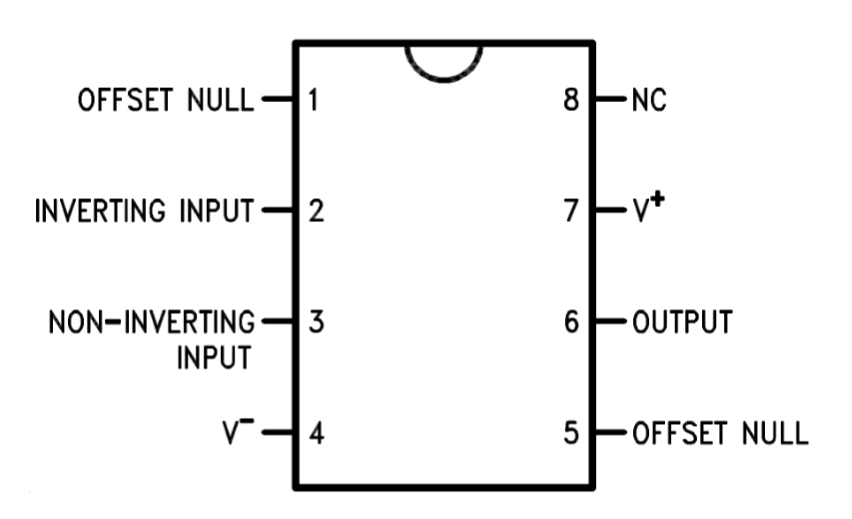
\includegraphics[width=0.4\textwidth]{content/images/opvinputs.png}
    \caption{Darstellung der Steckplätze des Verwendeten Operationsverstärkers \cite{TI_LM741_2025}.}
    \label{fig:opvinputs}
\end{figure}
\subsection{Der ideale und reale Operationsverstärker}
Der ideale Operationsverstärker hat einen unendlich großen Eingangswiderstand und sein Ausgangswiderstand beträgt $R=\qty{0}{\ohm}$. 
Die Verstärkung sowie die Bandbreite der Übertragung ist also unendlich groß. 
Bei einem realen Operationsverstärker kann dies nicht der Fall sein.  
Die Widerstände sind endlich: Meist liegt der Eingangswiderstand bei $> \qty{1}{\mega\ohm}$ und der Ausgangswiderstand bei $10 \,  \mathrm{bis} \, \qty{1000}{\ohm}$.
Er kann Verstärkungen von ca. $10^4$ bis $10^6$ erreichen. 
Die Bandbreite ist ebenfalls nach oben beschränkt, da die Transistoren im Operationsverstärker nicht unendlich schnell schalten können \cite[2]{federau_2017}. 






%fehlt noch: gegenkopplung -> lineare Verstärkung -> Kennlinie
\subsection{Kennlinie eines Operationsverstärkers}
Eine typische Kennlinie eines Operationsverstärkers von Ein- und Ausgangsspannung ist beispielhaft in \autoref{fig:kennlinie} zu erkennen. 
Dabei wird deutlich, dass die Verstärkung zunächst linear ist, wie bereits aus \autoref{equ:verstaerkung} hervorgeht. 
Ist nun aber die theoretisch erreichte Ausgangsspannung größer als die Versorgungsspannung, steigt die Ausgangsspannung natürlich nicht weiter, sondern bleibt auf ihrem maximalen Wert.
Auch dies ist in der Kennlinie deutlich zu erkennen. 
\begin{figure}
    \centering
    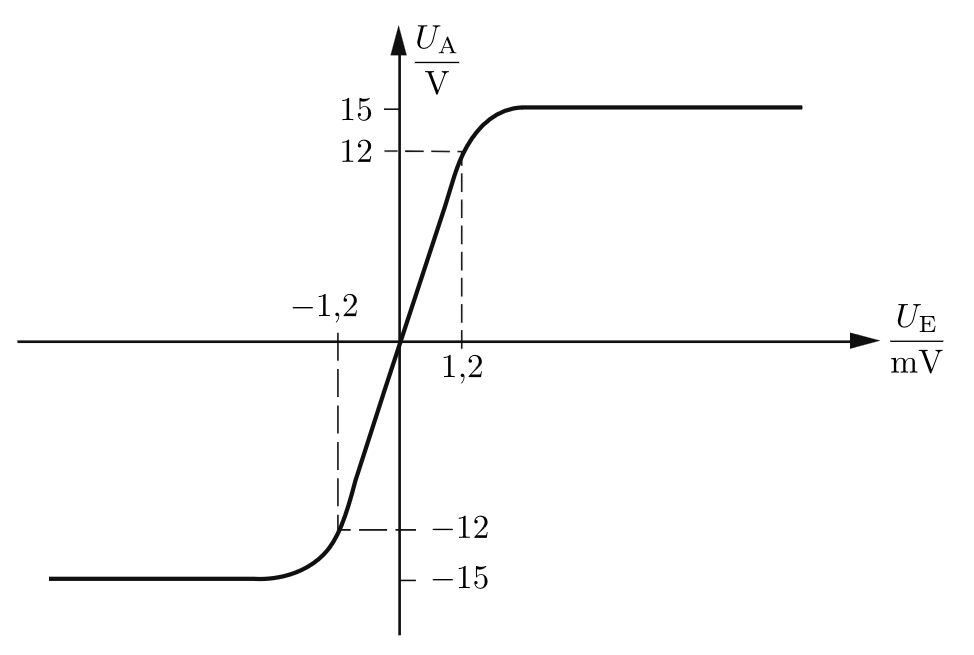
\includegraphics[width=0.7\textwidth]{content/images/kennlinie.png}
    \caption{Beispiel einer typischen Kennlinie eines Operationsverstärkers \cite{haas_2022}.}
    \label{fig:kennlinie}
\end{figure}



%--------------------------------------------------------------------------------------------------

\section{Verwendete Schaltungen mit dem Operationsverstärker}
\label{sec:schaltungen}
In diesem Versuch werden die vier in diesem Abschnitt folgenden Schaltungen aufgebaut und näher untersucht.
Dabei kann der Operationsverstärker nun als Blackbox angenommen werden. 
\subsection{Invertierender Linearverstärker}
Die einfachste hier verwendete Schaltung ist der invertierende Linearverstärker mit Gegenkopplung, wie er in \autoref{fig:schalt1} dargestellt ist.
Die Schaltung zeichnet sich dadurch aus, dass der Ausgang mit dem invertierenden Eingang über einen Widerstand verbunden ist. 
Daher wird von einer Gegenkopplung gesprochen. 
Diese sorgt wiederum dafür, dass die Verstärkung des Operationsverstärkers abflacht, da durch die Kopllung des Ausgangs an den invertierenden Eingang, die Spannungsdifferenz am Eingang verringert wird.
Somit vergrößert sich der Bereich der Eingangsspannung, in dem die Verstärkung linear ist und noch nicht ihren Grenzwert erreicht hat. 
So kann mit dieser Schaltung die Verstärkung des Operationsverstärkers ermittelt werden. 
\begin{figure}
    \centering
    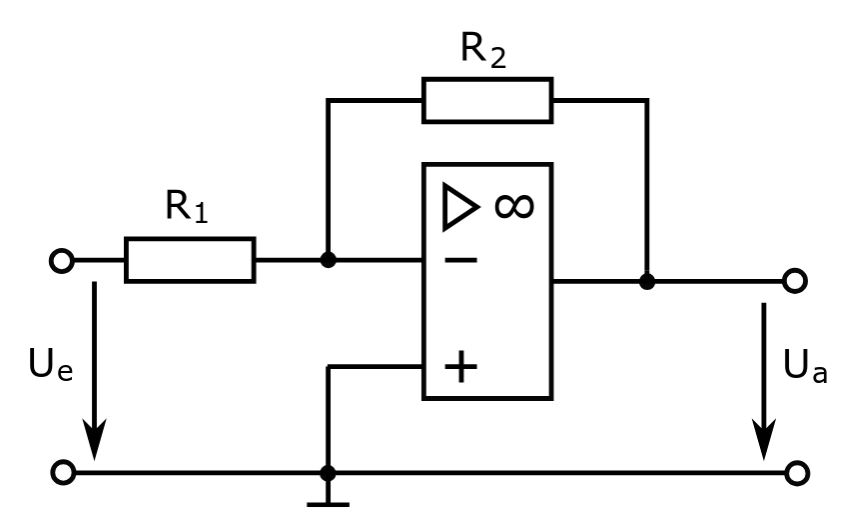
\includegraphics[width=0.5\textwidth]{content/images/schalt1.png}
    \caption{Schaltung eines invertierenden Linearverstärkers mit dem Operationsverstärker \cite{V51}.}
    \label{fig:schalt1}
\end{figure}
Mit dem Ohmschen Gesetzt ergibt sich aus \autoref{equ.verstaerkung} dann
\begin{equation}
    A = \frac{U_{\mathrm{a}}}{U_{\mathrm{e}}} = \frac{R_2}{R_1}
\end{equation}
für die Verstärkung des Operationsverstärkers, da durch beide Widerstände der gleiche Strom fließen muss. 

\subsection{Umkehr-Integrator}
Die Schaltung in \autoref{fig:schalt2} ist ein Umkehr-Integrator. 
Das Ausgangssignal ist also die Stammfunktion des Eingangssignals.
Hierbei ist nun anstelle von zwei Widerständen ein Widerstand und ein Kondensator verbaut.  
\begin{figure}
    \centering
    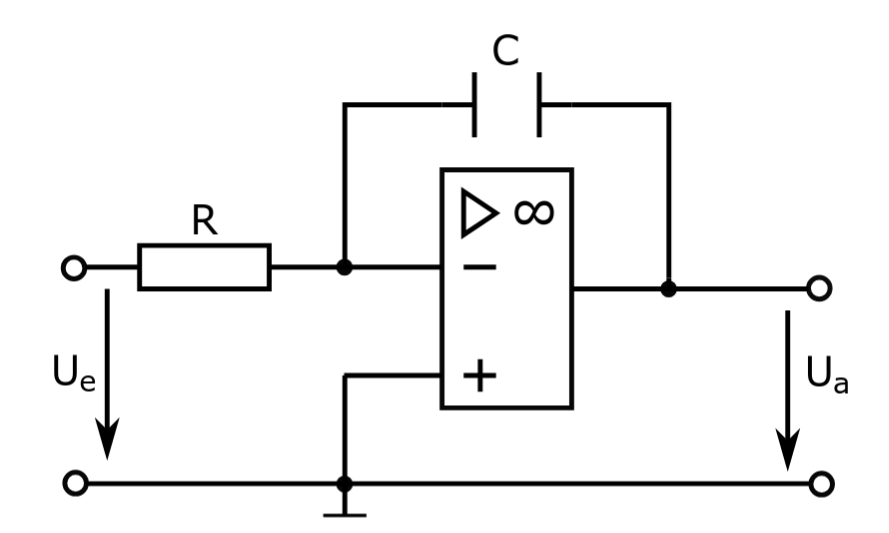
\includegraphics[width=0.5\textwidth]{content/images/schalt2.png}
    \caption{Schaltung eines Umkehr-Integrators mit dem Operationsverstärker \cite{V51}.}
    \label{fig:schalt2}
\end{figure}
Warum die Schaltung diese Eigenschaft hat, wird durch folgendes deutlich: 
Für den Strom am Widerstand $R$ und am Kondensator $C$ gilt jeweils: \textbf{QUELLE?}
\begin{align*}
    I_{\mathrm{R}}=\frac{U_{\mathrm{e}}}{R} & & I_{\mathrm{C}} = C \frac{\mathrm{d} U_{\mathrm{a}}}{\mathrm{d} t} \, .
\end{align*}
Wegen der Knotenregel müssen beide Ströme gleich sein. Gleichsetzen und Umformen liefert somit den Zusammenhang 
\begin{equation}
    U_{\mathrm{a}}\left(t\right) = - \frac{1}{RC}\int U_{\mathrm{e}}\left(t\right) \, \mathrm{d} \nonumber
\end{equation}
zwischen Ein- und Ausgangsspannung. Somit ist zu erkennen, dass die Schaltung tatsächlich das Eingangssignal integriert. 
Liegt hier am Eingnag eine Wechselstromspannung an, dann ergibts sich der Zusammenhang
\begin{equation}
    A \propto \frac{1}{f}
    \label{equ:fint}
\end{equation}
zwischen der Verstärkung und der Frequenz $f$ des Eingangssignals.

\subsection{Invertierender Differenzierer}
Werden Kondensator und Widerstand in der vorherigen Schaltung vertauscht, dann leitet die resultierende Schaltung das Eingangssignal ab. 
Die Schaltung ist ein invertierender Differenzierer und in \autoref{fig:schalt3} zu erkennen. 
\begin{figure}
    \centering
    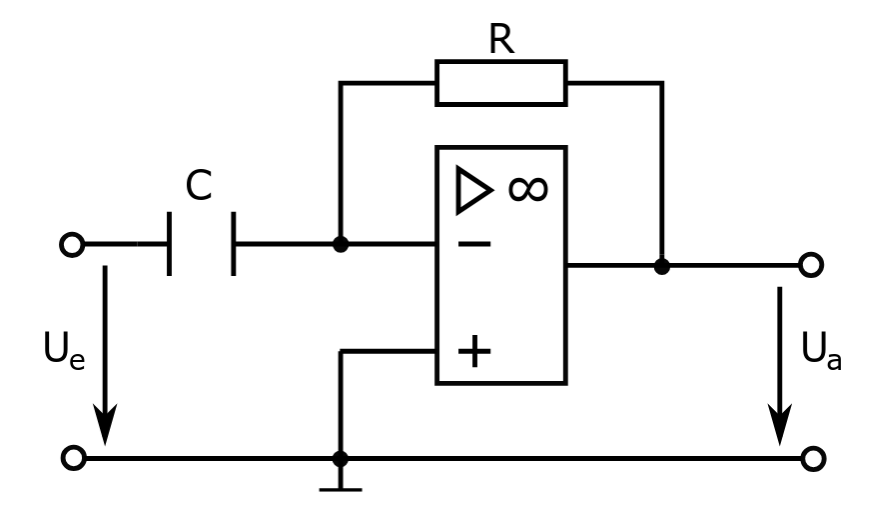
\includegraphics[width=0.5\textwidth]{content/images/schalt3.png}
    \caption{Schaltung eines invertierenden Differenzierers mit dem Operationsverstärker \cite{V51}.}
    \label{fig:schalt3}
\end{figure}
Durch ähnliches Vorgehen, wie bei dem Umkehr-Integrator wird klar, warum diese Schaltung ein Differenzierer ist:
Erneut gilt am Kondensator $C$ und am Widerstand $R$ jeweils: \textbf{QUELLE?}
\begin{align*}
     & & I_{\mathrm{C}} = C \frac{\mathrm{d} U_{\mathrm{e}}}{\mathrm{d} t} & & I_{\mathrm{R}}=\frac{U_{\mathrm{a}}}{R} \, . 
\end{align*}
Daraus ergibt sich bei dieser Schaltung allerdings
\begin{equation}
    U_{\mathrm{a}}\left(t\right) = - RC \frac{\mathrm{d} U_{\mathrm{e}}}{\mathrm{d} t}\, , \nonumber
\end{equation}
da Widerstand und Kondensator im Vergleich zum Umkehr-Integrator vertauscht sind.
Dies zeigt, dass bei dieser Schaltung das Ausgangssignal der Ableitung des Eingangssignals entspricht.
Hierbei ergibt sich bei Anliegen einer Wechselstromspannung nun allerdings 
\begin{equation}
    A \propto f
    \label{equ:fdiff}
\end{equation}
als Proportionalität.

\subsection{Schmitt-Trigger}
Eine weitere Schaltung ist der in \autoref{fig:schalt4} dargestellte Schmitt-Trigger.
\begin{figure}
    \centering
    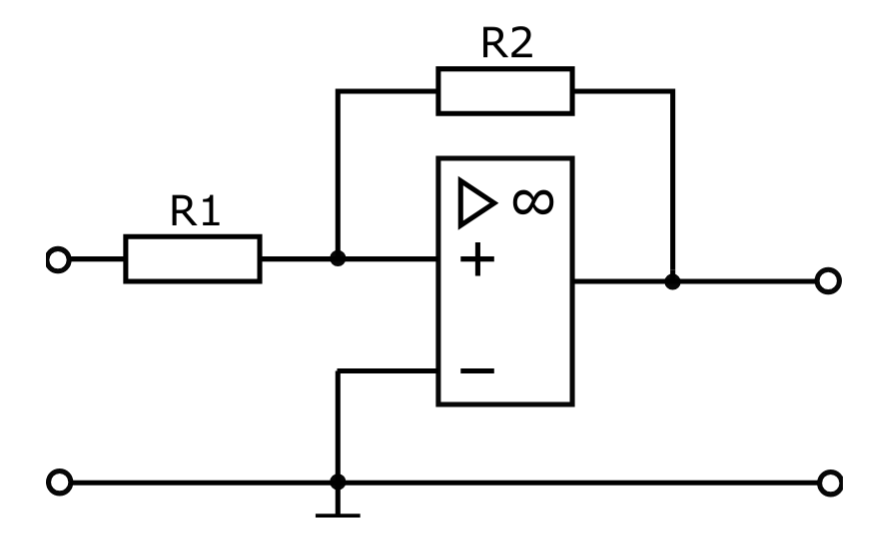
\includegraphics[width=0.5\textwidth]{content/images/schalt4.png}
    \caption{Schaltung eines Schmitt-Triggers mit dem Operationsverstärker \cite{V51}.}
    \label{fig:schalt4}
\end{figure} 
Der Aufbau ist ähnlich wie beim Linearverstärker, allerding wird statt einer Gegenkopplung nun eine Mitkopplung verwendet.
Das heißt, dass heir der Ausgang statt an den invertierenden Eingang an den nicht-invertierenden Eingang gekoppelt ist.
Dadurch tritt der genau entgegengesetzte Effekt, wie bei der Gegenkopplung des Linearverstärkers auf.
Die Steigung im Bereich der Linearen Verstärkung wird so stark, dass die Schaltung sofort die positive oder negative maximale Ausgangsspannung ausgibt.
Dabei gibt es für die eingehende Spannungsdifferenz eine Schwelle, ab der der Schmitt-Trigger in das jeweils andere Maximum wechselt.
Dieses Kippverhalten wird auch anhand der Kennlinie der Schaltung - die sogenannte Hysterese -, wie sie in \autoref{fig:hysterese} zu erkennen ist, deutlich.
Die Schwellspannung ab der die Schaltung jeweils Kippt ist durch
\begin{equation}
    U_{\mathrm{Schwelle}} = \pm \left|U_{\mathrm{a,max}}\right| \frac{R_1}{R_1+R_2}
    \label{equ:fdiff}
\end{equation}
gegeben \cite[126]{haas_2022}.
\begin{figure}
    \centering
    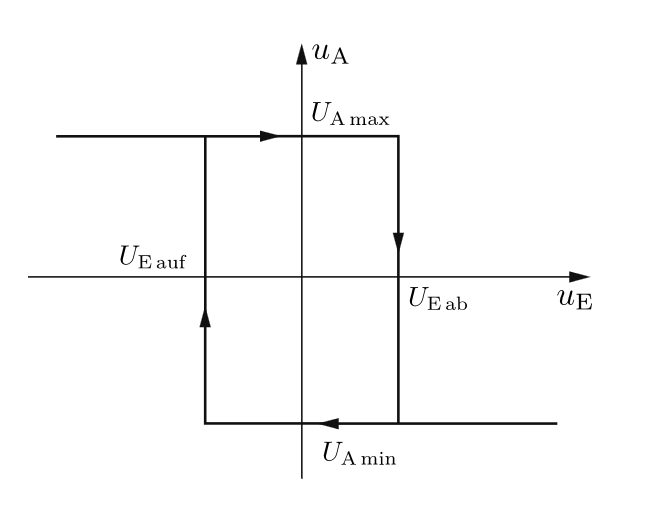
\includegraphics[width=0.5\textwidth]{content/images/hysterese.png}
    \caption{Schematische Darstellung der Hysterese bzw. der Kennlinie eines Schmitt-Triggers mit minimaler bzw. maximaler Amplitude $U_{\mathrm{A\,min}}$ und $U_{\mathrm{A\,max}}$ sowie den Schwellspannungen $U_{\mathrm{E \, auf}}$ und $U_{\mathrm{E \, ab}}$ \cite[125]{haas_2022}.}
    \label{fig:hysterese}
\end{figure}
